%%
%% This is file `tikzposter-template.tex',
%% generated with the docstrip utility.
%%
%% The original source files were:
%%
%% tikzposter.dtx  (with options: `tikzposter-template.tex')
%%
%% This is a generated file.
%%
%% Copyright (C) 2014 by Pascal Richter, Elena Botoeva, Richard Barnard, and Dirk Surmann
%%
%% This file may be distributed and/or modified under the
%% conditions of the LaTeX Project Public License, either
%% version 2.0 of this license or (at your option) any later
%% version. The latest version of this license is in:
%%
%% http://www.latex-project.org/lppl.txt
%%
%% and version 2.0 or later is part of all distributions of
%% LaTeX version 2013/12/01 or later.
%%


\documentclass{tikzposter} %Options for format can be included here

\usepackage{todonotes}

\usepackage[tikz]{bclogo}
\usepackage{lipsum}
\usepackage{amsmath}

\usepackage{booktabs}
\usepackage{longtable}
\usepackage[absolute]{textpos}
\usepackage[it]{subfigure}
\usepackage{graphicx}
\usepackage{cmbright}
%\usepackage[default]{cantarell}
%\usepackage{avant}
%\usepackage[math]{iwona}
\usepackage[math]{kurier}
\usepackage[T1]{fontenc}


%% add your packages here
\usepackage{hyperref}
% for random text
\usepackage{lipsum}
\usepackage[english]{babel}
\usepackage[pangram]{blindtext}

\colorlet{backgroundcolor}{blue!10}

 % Title, Author, Institute
\title{FLIP 00 PROJECT REPORT}
\author{Bing Liu$^1$}
\institute{$^1$ Jilin University, China \\
	$^2$ Deakin University, Australia
}
%\titlegraphic{logos/tulip-logo.eps}

%Choose Layout
\usetheme{Wave}

%\definebackgroundstyle{samplebackgroundstyle}{
%\draw[inner sep=0pt, line width=0pt, color=red, fill=backgroundcolor!30!black]
%(bottomleft) rectangle (topright);
%}
%
%\colorlet{backgroundcolor}{blue!10}

\begin{document}


\colorlet{blocktitlebgcolor}{blue!23}

 % Title block with title, author, logo, etc.
\maketitle

\begin{columns}
 % FIRST column
\column{0.5}% Width set relative to text width

%%%%%%%%%% -------------------------------------------------------------------- %%%%%%%%%%
 %\block{Main Objectives}{
%  	      	\begin{enumerate}
%  	      	\item Formalise research problem by extending \emph{outlying aspects mining}
%  	      	\item Proposed \emph{GOAM} algorithm is to solve research problem
%  	      	\item Utilise pruning strategies to reduce time complexity
%  	      	\end{enumerate}
%%  	      \end{minipage}
%}
%%%%%%%%%% -------------------------------------------------------------------- %%%%%%%%%%


%%%%%%%%%% -------------------------------------------------------------------- %%%%%%%%%%
\block{Introduction}{
    This is a demand forecasting problem. Participants are asked to combine historical usage patterns with weather data in order to forecast bike rental demand in the Capital Bike share program in Washington, D.C. Data is provided as follow.\\
    \begin{itemize}
		\smallskip
		\item \textbf{train.csv} -- it contains 10886 rows and 12 columns. Each row represents bike rental data for a certain hour. Each column indicates the current conditions
		\smallskip
		\item \textbf{test.csv} -- it contains 6493 rows and 9 columns. Compared with the train data, there are fewer "casual","registered" and "count" columns.
		\smallskip
		\item \textbf{sampleSubmission.csv} -- it clarifies the data submission format. It just contains 2 columns that is "datetime" and "count".
	\end{itemize}
}
%%%%%%%%%% -------------------------------------------------------------------- %%%%%%%%%%


%%%%%%%%%% -------------------------------------------------------------------- %%%%%%%%%%
\block{Data processing}{
\begin{itemize}
    \item \textbf{Missing values analysis} Use "missingno" to visualize missing value in the dataset. \\
    \item \textbf{Outliers analysis} Analyze the relationship between demand and date, season, hour of the day, and working day or not. \\
    \item \textbf{Correlation analysis} Analyze the correlation between count and temp, atemp, humidity and windspeed. \\
\end{itemize}
}
%%%%%%%%%% -------------------------------------------------------------------- %%%%%%%%%%


%%%%%%%%%% -------------------------------------------------------------------- %%%%%%%%%%

%\note{Note with default behavior}

%\note[targetoffsetx=12cm, targetoffsety=-1cm, angle=20, rotate=25]
%{Note \\ offset and rotated}

 % First column - second block


%%%%%%%%%% -------------------------------------------------------------------- %%%%%%%%%%
\block{Data Visualization}{
    Data visualization of the relationship between demand and date, season, hour of the day, and working day or not is follow, which show some information about data feature.
\begin{tikzfigure}%[Overall architecture of \emph{GOAM} algorithm]
    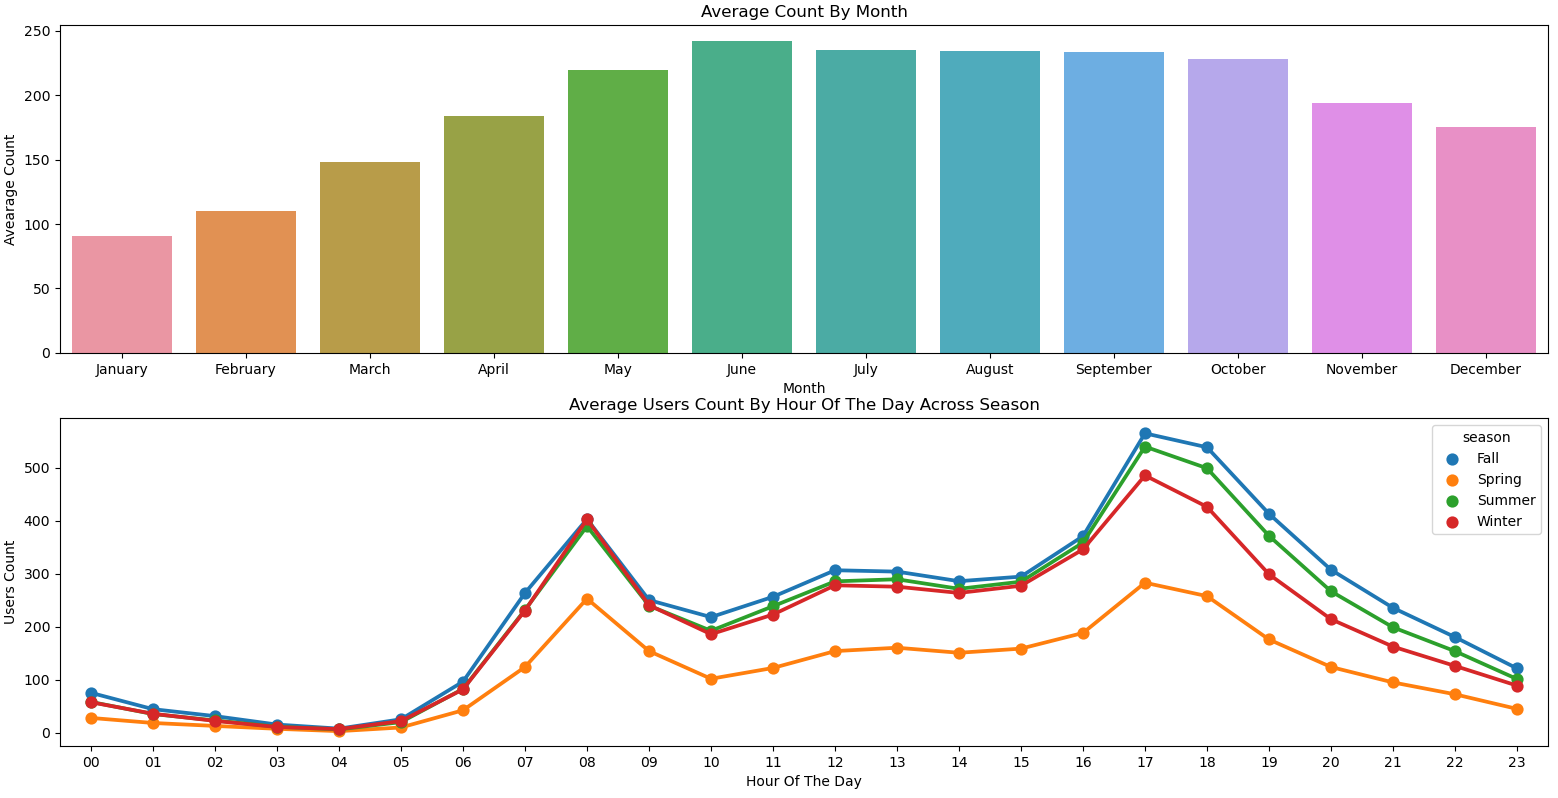
\includegraphics[width=0.8\linewidth]{logos/Figure_6.eps}
    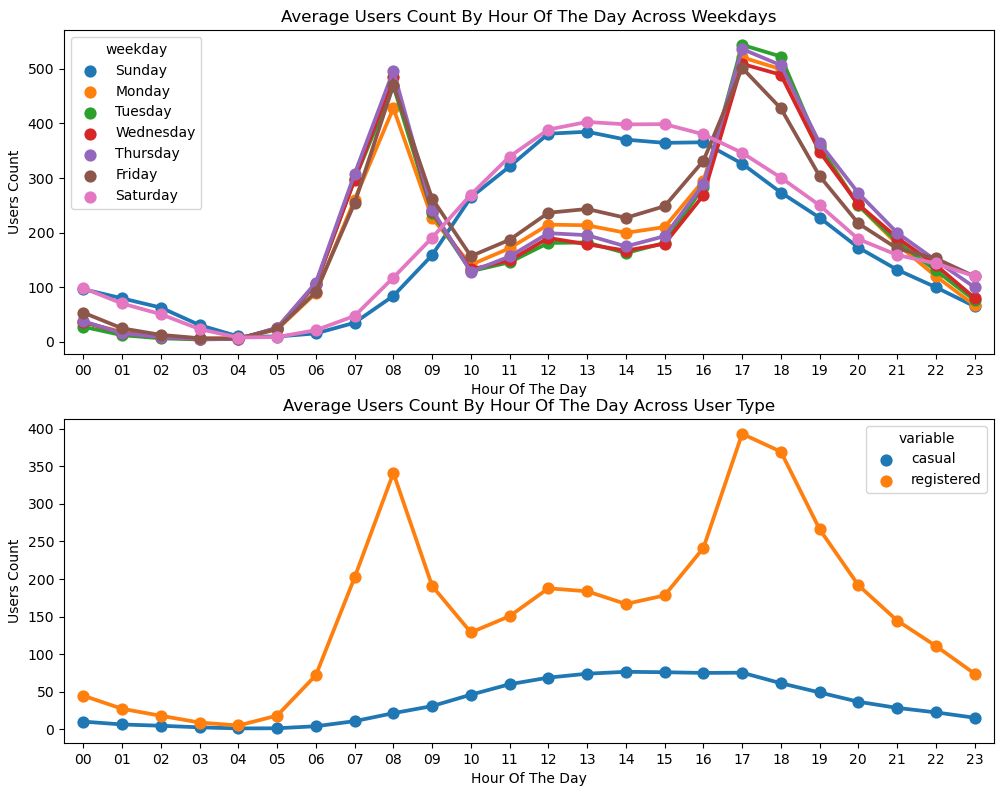
\includegraphics[width=0.8\linewidth]{logos/Figure_7.eps}
\end{tikzfigure}

%    1) Group Feature Extraction,
%    2) Outlying Degree Scoring, and
%    3) Outlying Aspects Identification.
  

}
%%%%%%%%%% -------------------------------------------------------------------- %%%%%%%%%%


% SECOND column
\column{0.5}
 %Second column with first block's top edge aligned with with previous column's top.

%%%%%%%%%% -------------------------------------------------------------------- %%%%%%%%%%
\block{Feature Engineering}{
\begin{itemize}
    \item \textbf{Time feature processing} Split the given date into "date, hour, year, weekday, month". \\
    \item \textbf{Feature selection} According to the data analysis results, select the more relevant features as the input data of the training model. The significant features contain temp, humidity, windspeed, atemp. \\
    \item \textbf{Training set and test set division} Divide train set and test set according to whether there is count attribute. \\
\end{itemize}
}
%%%%%%%%%% -------------------------------------------------------------------- %%%%%%%%%%
% Second column - first block


%%%%%%%%%% -------------------------------------------------------------------- %%%%%%%%%%
\block[titleleft]{Model and Experiment}
{
I have choose the Ensemble Model - Gradient Boost. Compare the distribution of train and test results.It confirms visually that the model has not predicted really bad and not suffering from major overfitting problem.
\begin{tikzfigure}%[Overall architecture of \emph{GOAM} algorithm]
    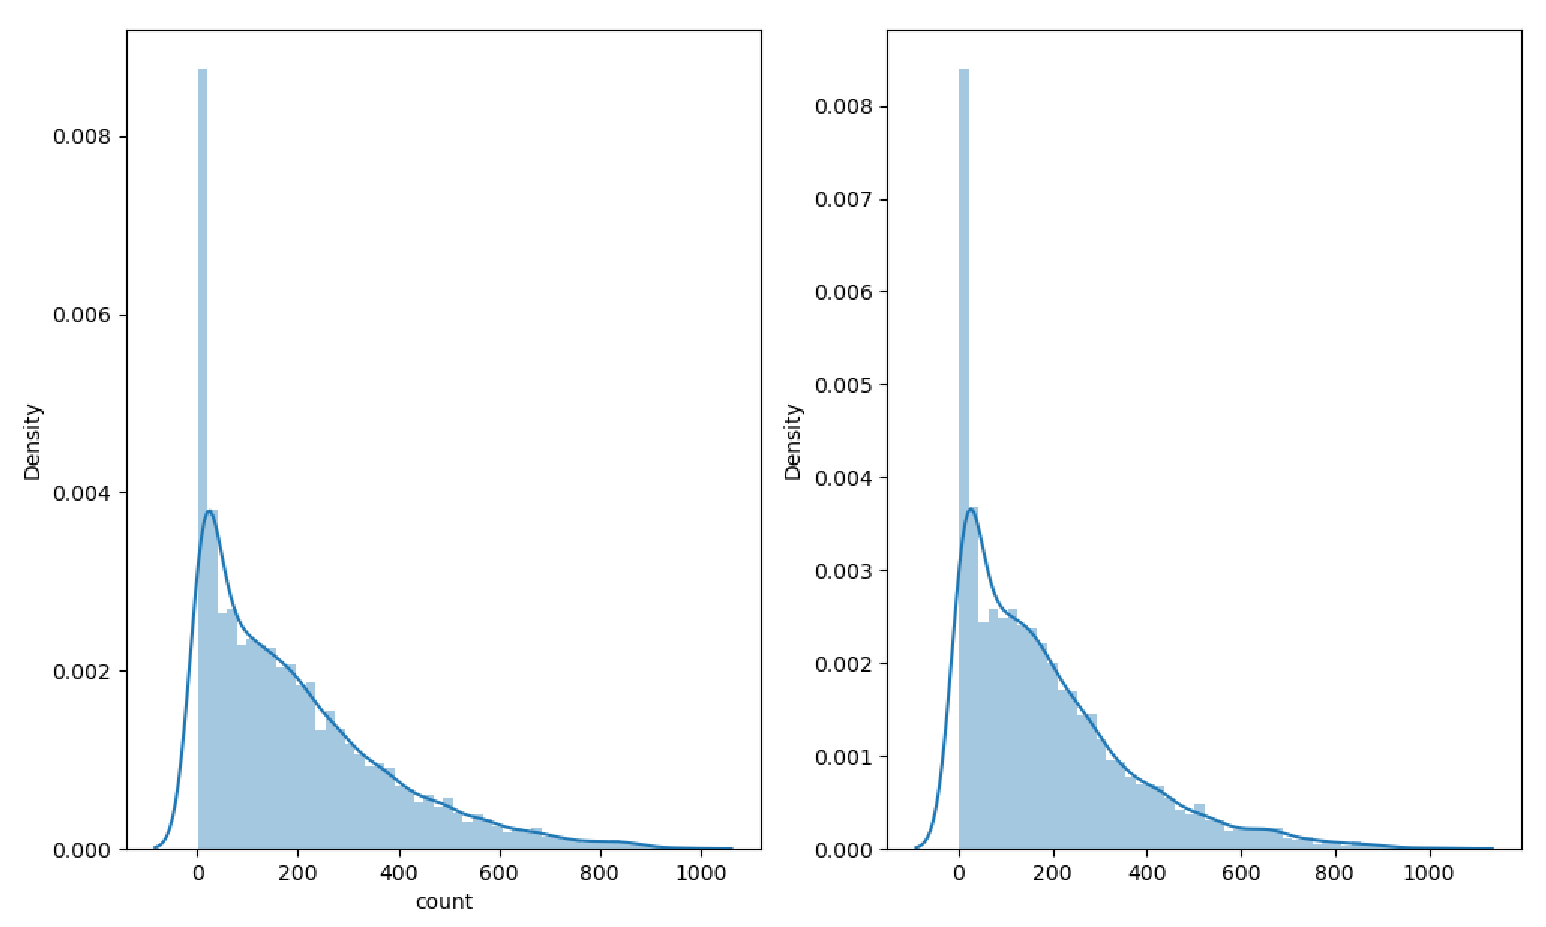
\includegraphics[width=0.8\linewidth]{logos/models_Figure_1.eps}
\end{tikzfigure}
}
%%%%%%%%%% -------------------------------------------------------------------- %%%%%%%%%%


% Second column - second block
%%%%%%%%%% -------------------------------------------------------------------- %%%%%%%%%%
\block[titlewidthscale=1, bodywidthscale=1]
{Conclusion}
{
\begin{description}
  \item[Loss function] 
  Using RMSLE to calculate the error, it penalizes under-prediction even more.

  \item[RMSLE Value]
  RMSLE Value For Gradient Boost: 0.189973542608

  \item[Rank]
  The score of my submission in kaggle is 0.41867. Ranked 428 among 3242 teams.

\end{description}
}
%%%%%%%%%% -------------------------------------------------------------------- %%%%%%%%%%


% Bottomblock
%%%%%%%%%% -------------------------------------------------------------------- %%%%%%%%%%
\colorlet{notebgcolor}{blue!20}
\colorlet{notefrcolor}{blue!20}
%\note[targetoffsetx=8cm, targetoffsety=-4cm, angle=30, rotate=15,
\note[targetoffsetx=8cm, targetoffsety=-21cm, angle=30, rotate=15,
radius=2cm, width=.26\textwidth]{
Acknowledgement
\begin{itemize}
    \item
    Flip00 project report, 26/04/2021, changchun. China
 \end{itemize}
}

%\note[targetoffsetx=8cm, targetoffsety=-10cm,rotate=0,angle=180,radius=8cm,width=.46\textwidth,innersep=.1cm]{
%Acknowledgement
%}

%\block[titlewidthscale=0.9, bodywidthscale=0.9]
%{Acknowledgement}{
%}
%%%%%%%%%% -------------------------------------------------------------------- %%%%%%%%%%

\end{columns}


%%%%%%%%%% -------------------------------------------------------------------- %%%%%%%%%%
%[titleleft, titleoffsetx=2em, titleoffsety=1em, bodyoffsetx=2em,%
%roundedcorners=10, linewidth=0mm, titlewidthscale=0.7,%
%bodywidthscale=0.9, titlecenter]

%\colorlet{noteframecolor}{blue!20}
\colorlet{notebgcolor}{blue!20}
\colorlet{notefrcolor}{blue!20}
\note[targetoffsetx=-13cm, targetoffsety=-34cm,rotate=0,angle=180,radius=8cm,width=.96\textwidth,innersep=.4cm]
{
\begin{minipage}{0.3\linewidth}
\centering

\includegraphics[width=24cm]{logos/tulip-wordmark.eps}
\end{minipage}
\begin{minipage}{0.7\linewidth}
{ \centering
  Flip00 project report,
  Latex and Git,
  26/04/2021, Changchun, China
}
\end{minipage}
}
%%%%%%%%%% -------------------------------------------------------------------- %%%%%%%%%%


\end{document}

%\endinput
%%
%% End of file `tikzposter-template.tex'.
